\documentclass[conference]{IEEEtran}
\IEEEoverridecommandlockouts

\usepackage{cite}
\usepackage{amsmath,amssymb,amsfonts}
\usepackage{algorithmic}
\usepackage{graphicx}
\usepackage{textcomp}
\usepackage{xcolor}
\usepackage{booktabs}
\usepackage{tikz}
\usepackage{pgfplots}
\pgfplotsset{compat=1.17}
\usetikzlibrary{arrows.meta,positioning,shapes.geometric}

\def\BibTeX{{\rm B\kern-.05em{\sc i\kern-.025em b}\kern-.08em
    T\kern-.1667em\lower.7ex\hbox{E}\kern-.125emX}}

\begin{document}

\title{Vr-Hmt: Virtual Reality-Driven Human Motion Tracking System via Mask Rcnn for Real-Time Monitoring}

\author{
\IEEEauthorblockN{Kannan R}
\IEEEauthorblockA{\textit{Dept. of Electrical and Electronics Engineering} \\
\textit{Nehru Institute of Engineering and Technology}\\
Coimbatore, India \\
Kannan234@gmail.com}
\and
\IEEEauthorblockN{Suguna T}
\IEEEauthorblockA{\textit{Department of Information Technology} \\
\textit{Government College of Technology}\\
Coimbatore, Tamil Nadu, India \\
Suguna324@outlook.com}
\and
\IEEEauthorblockN{Sivasubramanian R}
\IEEEauthorblockA{\textit{Department of AIML} \\
\textit{Malla Reddy University}\\
Dulapally, Hyderabad, India \\
Sivasubramanian243@gmail.com}
\and
\IEEEauthorblockN{Bhuvanesh A}
\IEEEauthorblockA{\textit{Dept. of Electrical and Electronics Engineering} \\
\textit{PSN College of Engineering and Technology}\\
Tirunelveli, India \\
Bhuvanesh56@gmail.com}
\and
\IEEEauthorblockN{Vemulapalli Sri Lakshmi Harshitha}
\IEEEauthorblockA{\textit{Dept. of BE Computer Science and Design} \\
\textit{RMK Engineering College (autonomous)}\\
Kavaraipettai, Tamil Nadu, India \\
Vemulapalli82sri@gmail.com}
\and
\IEEEauthorblockN{Kulwant Singh}
\IEEEauthorblockA{\textit{Electronics And Communication Engineering} \\
\textit{Yadavindra Dept. of Engineering, Punjabi Univ. Guru Kashi Campus}\\
Talwandi Sabo, Distt. Bathinda \\
Kulwantsingh654@gmail.com}
\and
\IEEEauthorblockN{Chellam S}
\IEEEauthorblockA{\textit{Dept. of Electrical and Electronics Engineering} \\
\textit{Velammal College of Engineering and Technology}\\
Madurai, Tamil Nadu, India \\
Chellam342@gmail.com}
\and
\IEEEauthorblockN{Ahilan Appathurai}
\IEEEauthorblockA{\textit{Dept. of Electronics and Communication Engineering} \\
\textit{PSN College of Engineering and Technology}\\
Tirunelveli, Tamilnadu, India \\
Ahilan67@gmail.com}
}

\maketitle

\begin{abstract}
Human motion tracking (HMT) is capturing and analyzing the movement of individuals and objects, focusing on their location, speed, and acceleration. It is used in various fields including filmmaking, animation, sports analysis, robotics, and augmented reality. Unauthorized physical access to facilities presents significant challenges for organizations as it can result in theft, sabotage, and data breaches; these incidents lead to financial losses and compromised sensitive information. To overcome these challenges, a novel virtual reality (VR) based XXX system has been proposed for tracking human motion to identify any suspicious activity within an organization. The system uses various sensors such as cameras and motion sensors to capture real-world activity in a monitored space. These sensors capture continuous video, which has been converted into frames for further processing. The bilateral filter is used as a pre-processing step to minimize noise while maintaining edges in the frames. The Mask R-CNN model is used for HMT from the frames, assigns bounding boxes around each detected human, and predicts segmentation masks on each detected frame. The tracking data is stored in a database server and displayed on a large screen to observe the environment. The processed data is further transferred to an application server which serves as a control unit for managing the data and coordinating with the central platform. According to the result, the proposed model attains a 98.45\% accuracy rate for human motion tracking. The proposed XXX model achieves an overall accuracy improvement of 2.18\%, 8.99\%, and 1.47\% compared to the existing methods such as DBSCAN, cluster segmentation, and k-fold cross-validation.
\end{abstract}

\begin{IEEEkeywords}
Human motion tracking, Augmented reality, Virtual reality, bilateral filter, Mask R-CNN.
\end{IEEEkeywords}

\section{Introduction}

The term "human motion" describes the physical position of the human body changes over a day. Tracking and documenting the subject real-time 3D kinematics are possible with human motion analysis, an investigative diagnostic tool \cite{b1}. In many VR applications, including gaming and social interaction, HMT, which estimates the directions and positions of body joints in 3D space, is greatly desired \cite{b2}. Predicting a person's future poses based on their past motion history is known as human motion prediction. For applications like human tracking, human-robot interaction, and human motion synthesis for computer graphics, human motion prediction can be quite helpful \cite{b3}. To accurately detect motion, sensors must not only be robust and lightweight but also have a high level of sensitivity. Tensile force, pressure, and other characteristics are detected by these sensors, which are categorized into capacitive, piezoelectric, resistive, and triboelectric varieties based on their sensing processes. Of these, resistive sensors have attracted a lot of interest because of their comparatively straightforward operation, workable manufacturing procedures, and simplicity of signal gathering \cite{b4}.

Modern electronics and sophisticated data processing across various sense modalities, such as aural, visual, tactile, somatosensory, and olfactory integrate the virtual and physical worlds to create AR, an interactive experience. VR is an immersive computer-generated world in which users interact with virtual objects. Because of haptic technology, VR can also provide additional forms of physical feedback in addition to aural and visual feedback \cite{b5}. Applications for AR and VR have exciting possibilities. Some of the more innovative uses include virtual meeting spaces, collaborative works, and world-navigating personal assistants. Although it is obvious that merging the physical and virtual realms is essential for an immersive experience, the existing AR/VR experience is limited to small spaces, or, more generally, a few square meters that may or may not be devoid of things. However, think about routine tasks like arranging furniture around a table, opening and closing doors, and moving between rooms. The limitations of current technology make it difficult to capture even these basic actions, which restricts the potential uses of AR and VR \cite{b6}.

For both VR and non-VR applications, VR motion tracking tools have shown to be a viable motion tracking solution including medical science, motion simulators, robotics, science, motion capture, mixed reality film production, rehabilitation, and interactive art. Custom motion tracking technologies, including the Oculus sensor, VLTS, and camera-based, insight tracking are made by each VR consumer product manufacturer \cite{b7}. Three primary steps can be used to identify tracking algorithms in general: choosing the right image features, modeling the item's shape, appearance, and motion, and representing the intended object for visual tracking \cite{b8,b9}. Accurately anticipating human mobility is a difficult endeavor because the way people act is complicated and influenced by a variety of internal and external factors. The intention of one's own goals, the incidence and behavior of other agents nearby, the social relationships between agents, social laws and conventions, geometry, semantics, topology, and affordances can all influence motion behavior \cite{b10}. The HMP challenge, which has several applications in fields like autonomous driving and healthcare, is to predict potential future pose sequences from a sequence of observed motions. Due to the constant requirement that the projected motions be continuous, varied, and realistic at the same time, this challenge is difficult and demanding \cite{b11}.

The key contributions are as follows,
\begin{itemize}
\item The primary purpose of this research is to design a novel virtual reality (VR) based XXX system that has been proposed for detecting suspicious activity within an organization.
\item The system uses various sensors such as cameras and motion sensors to capture real-world activity in a monitored space. These sensors capture continuous video, that video has been converted into frames for further processing.
\item The video frames are pre-processed using the bilateral filter to reduce noise while preserving edges.
\item The Mask R-CNN model is used for human motion tracking from the frames, assigns bounding boxes around each detected human and predicts segmentation masks on each detected frame.
\end{itemize}

The structure of the paper is organized as follows: Section II briefly explains the literature survey, the proposed Mask RCNN is explained in Section III, the performance results and their comparison analysis are provided in Section IV, and Section V encloses a conclusion and future work.

\section{Literature Survey}

In recent years, several researchers have investigated human motion tracking with DL and ML methods. The section that follows provides a review of some current research papers.

In 2024, Shen, Z., et al. \cite{b12} suggested a system for fall detection and real-time tracking that is intended for numerous human targets. They performed a thorough analysis with more than 300 minutes of data or over 360,000 frames. Furthermore, the system shows a high accuracy rate of 96.3\% in the field of human fall detection, highlighting its efficacy in differentiating falls from other states.

In 2023, Boonsongsrikul, A. and Eamsaard, J. \cite{b13} proposed a Tello EDU drone-based human motion tracking technique. Four steps comprise the design methodology: notification systems, HMT algorithm, control panel design, and communication and distance extension. With an aggregate tracking length of 84.30 meters and a top vertical monitoring length of 13.40 meters, the flying machine was operated from a laptop connected to a Wi-Fi connection. The experiment revealed a human movement detection accuracy rate ranging from 96.67\% to 100\%.

In 2016, Liu, Z., et al. \cite{b14} proposed a technique for capturing human motion that relies on a network of inexpensive RGBD cameras working together. Three cameras were used to record a wide range of human behaviors in indoor environments in order to confirm the approach's robustness and efficiency.

In 2018, Seemanthini, K. and Manjunath, S.S. \cite{b15} proposed a temporal tracking method and hierarchical graph-based segmentation for a human action recognition system. The SVM algorithm was used for classification, and each object's activity was identified from the classification outcome. The suggested model computes an accuracy of up to 89.59\% for each object's detection.

In 2020, Wilk, M.P., et al. \cite{b16} proposed a low-cost solution in the form of a prototype opto-inertial motion tracking system. The 3D position is determined by combining data from optical and inertial sensors with details about two external reference sites using a data fusion technique and direction. The total RMSE in location and direction, according to the data, was 32.8 mm and 0.89 degrees, respectively.

In 2024, Khan, D., et al. \cite{b17} proposed a robust system that can efficiently recognize human movement and localization activities using the k-fold cross-validation method, combining information from two external reference locations with data from optical and inertial sensors.

In 2020, Aalerud, A. and Hovland, G. \cite{b18} proposed 3D sensors to track human mobility in real time. By dynamically including 3D sensors that offer reliable human location data in the Kalman filter, the suggested technique can handle occlusions. A 20 Hz frame rate, 50 ms to 100 ms latency, and 0.10 m to 0.15 m estimation precision were all achieved.

In 2021, Nallasivam, M. and Senniappan, V. \cite{b19} proposed an approach to tracking and detecting moving human targets. Under three distinct illumination situations, the suggested technique demonstrated superior performance in terms of precision, F1 score, accuracy, and recall.

In 2020, Patil, A.K., et al. \cite{b20} suggested a 3D light detection and inertial measurement unit (IMU) and ranging (lidar) sensor-based pose-tracking system. The findings show that the height and position estimation accuracy are both well within a reasonable range of $\pm$3-5 cm.

In 2021, Yue, S. \cite{b21} proposed a recursive tracking algorithm for human motion that is AR-oriented, integrating the Kanade-Lucas-Tomasi (KLT) algorithm and the oriented FAST and rotated BRIEF (ORB). Findings from experiments reveal that the recursive tracking method outperforms the detection tracking system in terms of time and accuracy.

Based on the above literature survey, existing techniques were developed using various DL and ML approaches to tracking human motion. However, these methods fail to provide a high reliability rate, and the process of human motion tracking needs more time. To address this challenge, a novel virtual reality-based XXX model has been proposed for tracking human motion to identify any suspicious activity within an organization.

\section{Proposed System}

In this section, a novel VR-based XXX system has been proposed for detecting suspicious activity within an organization. The system uses various sensors such as cameras and motion sensors to capture real-world activity in a monitored space. These sensors capture continuous video, which has been converted into frames for further processing. The video frames are pre-processed using the bilateral filter to reduce noise while preserving edges. The Mask R-CNN model is used for HMT from the frames, assigns bounding boxes around each detected human, and predicts segmentation masks on each detected frame. Fig. 1 shows the proposed XXX methodology.

\begin{figure}[htbp]
\centering
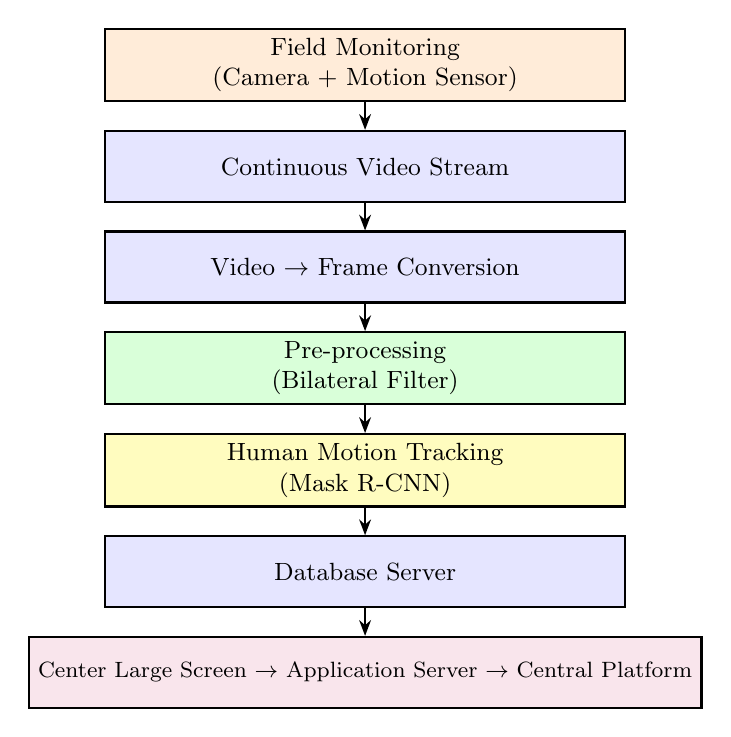
\begin{tikzpicture}[
  box/.style={rectangle, draw, thick, minimum width=6.6cm, minimum height=0.9cm, align=center, font=\small},
  arr/.style={-{Stealth[length=2mm]}, thick}
]
\node[box, fill=orange!15] (a) {Field Monitoring\\(Camera + Motion Sensor)};
\node[box, fill=blue!10, below=0.35cm of a] (b) {Continuous Video Stream};
\node[box, fill=blue!10, below=0.35cm of b] (c) {Video $\rightarrow$ Frame Conversion};
\node[box, fill=green!15, below=0.35cm of c] (d) {Pre-processing\\(Bilateral Filter)};
\node[box, fill=yellow!25, below=0.35cm of d] (e) {Human Motion Tracking\\(Mask R-CNN)};
\node[box, fill=blue!10, below=0.35cm of e] (f) {Database Server};
\node[box, fill=purple!10, below=0.35cm of f, minimum width=6.6cm] (g) {\footnotesize Center Large Screen $\rightarrow$ Application Server $\rightarrow$ Central Platform};
\draw[arr] (a) -- (b);
\draw[arr] (b) -- (c);
\draw[arr] (c) -- (d);
\draw[arr] (d) -- (e);
\draw[arr] (e) -- (f);
\draw[arr] (f) -- (g);
\end{tikzpicture}
\caption{The proposed XXX methodology}
\label{fig1}
\end{figure}

\subsection{Field monitoring}
A person wearing a headset monitors live video feeds through virtual reality glasses. This individual is likely involved in remote surveillance or monitoring of an area, using sensors for better insight. The deployed sensors are used for capturing real-time data in the surveillance system. Various sensors such as cameras and motion sensors capture real-world activity in a monitored space. The camera is used to capture video footage of the monitored area and constantly records and provides a video stream. Motion is recognized by a motion detector in the environment. When motion is encountered, the system can either set off alerts or begin recording through the camera, making it more efficient by focusing on human activity. The video footage is then broken down into individual frames for further analysis.

\subsection{Pre-processing}
The video frames are pre-processed using the bilateral filter to reduce noise while preserving edges, preparing the frames for human motion tracking. Fig. 2 displays the original image and the pre-processed image. The bilateral filter is a spatial domain filtering method for eliminating noise from images. To determine the value of a pixel, it takes into consideration both geometric and photometric proximity within a short neighborhood. The primary purpose of the bilateral filter is to eliminate additive Gaussian noise from images. In the filtering process, Gaussian distribution formulas are used to calculate the weights for geometric and photometric pixel closeness.

Equation~(1) illustrates the result of spatial domain filtering on a noisy input image,
\begin{equation}
h_1(x) = k_d^{-1}(x) \iint f(\epsilon)\,e(\epsilon,x)\,d\varepsilon
\end{equation}

The geometric distance between center $x$ and neighboring points $\epsilon$ is denoted by $e(\epsilon,x)$. Likewise, if filtering is performed with intensity changes in the small local window in mind, the result is shown by equation~(2).
\begin{equation}
h_2(x) = k_r^{-1}(x) \iint f(\epsilon)\,s(f(\epsilon),f(x))\,d\varepsilon
\end{equation}

Here, $s(f(\epsilon),f(x))$ is the photometric separation between neighboring points $\epsilon$ and center $x$. Utilizing a bilateral filter within a local window yields the outcome depicted in equation~(3), as this filter integrates both the spatial and intensity disparities among pixels within the window.
\begin{equation}
h(x) = k^{-1}(x) \iint f(\epsilon)\,s(f(\epsilon),f(x))\,d\varepsilon
\end{equation}

where the normalization constant is $k(x)$, shown in equation~(4).
\begin{equation}
K(x) = \iint e(\epsilon,x)\,s(f(\epsilon),f(x))\,d\varepsilon
\end{equation}

It is assumed that $e$ denotes geometric distance and $s$ denotes photometric distance in the normal bilateral filter, which is intended to eliminate additive Gaussian noise, provided by equations (5) and (6).
\begin{equation}
e(\epsilon,x) = \exp\left(\frac{-1}{2}\left(\frac{d(\epsilon,x)}{\sigma_d}\right)^2\right)
\end{equation}
\begin{equation}
s(\epsilon,x) = \exp\left(\frac{-1}{2}\left(\frac{d(f(\epsilon),f(x))}{\sigma_r}\right)^2\right)
\end{equation}

where the Euclidian distance is $d$.

\begin{figure}[htbp]
\centering
\fbox{\parbox[c][2.2cm]{0.9\linewidth}{\centering\itshape Insert image/screenshot here\\(original and pre-processed frame)}}
\caption{(a) Original image (b) Preprocessed image}
\label{fig2}
\end{figure}

\subsection{Human motion tracking}
The pre-processed frames are fed into the Mask R-CNN, which is developed from the Faster R-CNN model. Mask R-CNN comprises multiple architectures, namely a backbone architecture such as ResNet-50, a region proposal network (RPN), and region of interest (RoI) pooling. From the input images, a feature map is extracted by the backbone. Using the RPN, image regions that might contain objects are found. Following pooling, the regional proposals are presented as input data for object estimation to the fully connected MLP, allowing an estimate to be made among the predefined classes. Faster R-CNN produces faster results even though these processes are carried out more slowly than simpler detectors. Mask R-CNN emerged as a result of Faster R-CNN's development: Faster R-CNN ascertains each object's bounding box and class label during object detection, while Mask R-CNN additionally generates a segmentation mask for every item. Mask R-CNN uses a two-step process: in the first phase, the bounding boxes of the items are found using the region proposal network; in the second step, each object's mask is found using RoI Align. Fig. 3 displays the architecture of the Mask R-CNN.

\begin{figure}[htbp]
\centering
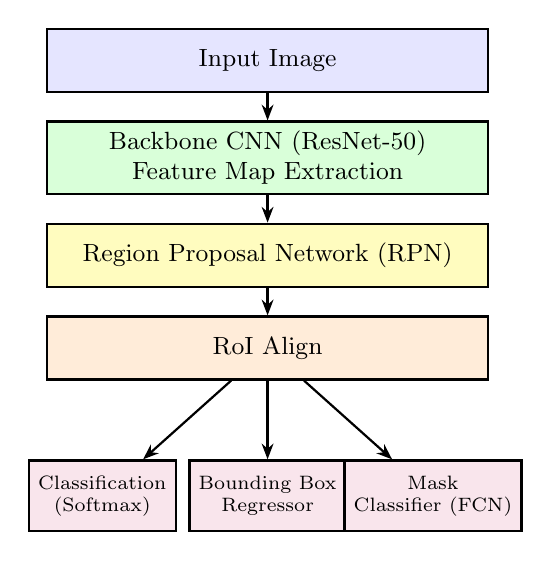
\begin{tikzpicture}[
  box/.style={rectangle, draw, thick, minimum width=5.6cm, minimum height=0.8cm, align=center, font=\small},
  sbox/.style={rectangle, draw, thick, minimum width=1.7cm, minimum height=0.9cm, align=center, font=\scriptsize},
  arr/.style={-{Stealth[length=2mm]}, thick}
]
\node[box, fill=blue!10] (a) {Input Image};
\node[box, fill=green!15, below=0.35cm of a] (b) {Backbone CNN (ResNet-50)\\Feature Map Extraction};
\node[box, fill=yellow!25, below=0.35cm of b] (c) {Region Proposal Network (RPN)};
\node[box, fill=orange!15, below=0.35cm of c] (d) {RoI Align};
\node[sbox, fill=purple!10, below=1.0cm of d, xshift=-2.1cm] (e1) {Classification\\(Softmax)};
\node[sbox, fill=purple!10, below=1.0cm of d] (e2) {Bounding Box\\Regressor};
\node[sbox, fill=purple!10, below=1.0cm of d, xshift=2.1cm] (e3) {Mask\\Classifier (FCN)};
\draw[arr] (a) -- (b);
\draw[arr] (b) -- (c);
\draw[arr] (c) -- (d);
\draw[arr] (d) -- (e1);
\draw[arr] (d) -- (e2);
\draw[arr] (d) -- (e3);
\end{tikzpicture}
\caption{The architecture of Mask R-CNN}
\label{fig3}
\end{figure}

\section{Results and Discussion}

This section shows the Fig. 4 evaluation of the suggested XXX model using the collected datasets, applying several measures consisting of specificity, F1 score, precision, recall, and accuracy. The benchmark includes the operation of the proposed result as well as the complete accuracy rate, which has been carefully defined and evaluated.

The system uses various sensors such as cameras and motion sensors to capture real-world activity in a monitored space. These sensors capture continuous video, which has been converted into frames for further processing. The frames are pre-processed using the bilateral filter to reduce noise while preserving edges. The Mask R-CNN model is used for HMT from the frames, assigns bounding boxes around each detected human, and predicts segmentation masks on each detected frame.

\begin{figure}[htbp]
\centering
\fbox{\parbox[c][2.2cm]{0.9\linewidth}{\centering\itshape Insert image/screenshot here\\(Mask R-CNN detection output)}}
\caption{Output of Mask R-CNN}
\label{fig4}
\end{figure}

\subsection{Performance analysis}
The proposed XXX model can be assessed based on specificity, precision, recall, accuracy, and F1 score.
\begin{equation}
Specificity = \frac{T_{neg}}{T_{neg}+F_{pos}}
\end{equation}
\begin{equation}
Precision = \frac{T_{pos}}{T_{pos}+F_{pos}}
\end{equation}
\begin{equation}
Recall = \frac{T_{pos}}{T_{pos}+F_{neg}}
\end{equation}
\begin{equation}
Accuracy = \frac{T_{pos}+T_{neg}}{\text{Total no. of samples}}
\end{equation}
\begin{equation}
F1\ score = 2\times\frac{Precision \times Recall}{Precision + Recall}
\end{equation}

where $T_{neg}$ and $T_{pos}$ specify the true negatives and true positives of the sample images, and $F_{neg}$ and $F_{pos}$ specify the false negatives and false positives of the sample images.

\begin{figure}[htbp]
\centering
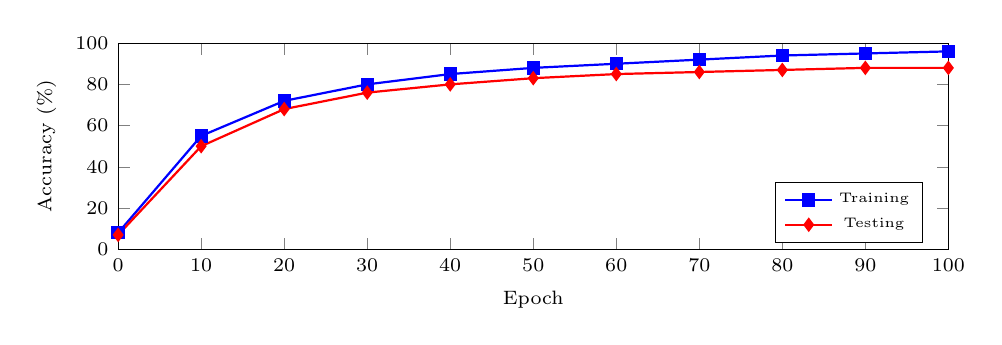
\begin{tikzpicture}
\begin{axis}[
  width=\linewidth, height=4.2cm,
  xlabel={Epoch}, ylabel={Accuracy (\%)},
  xmin=0, xmax=100, ymin=0, ymax=100,
  legend pos=south east, legend style={font=\tiny},
  label style={font=\scriptsize}, tick label style={font=\scriptsize}
]
\addplot[mark=square*, blue, thick] coordinates {
(0,8)(10,55)(20,72)(30,80)(40,85)(50,88)(60,90)(70,92)(80,94)(90,95)(100,96)
};
\addplot[mark=diamond*, red, thick] coordinates {
(0,7)(10,50)(20,68)(30,76)(40,80)(50,83)(60,85)(70,86)(80,87)(90,88)(100,88)
};
\legend{Training, Testing}
\end{axis}
\end{tikzpicture}
\caption{Training and testing accuracy curve of Mask R-CNN}
\label{fig5}
\end{figure}

\begin{figure}[htbp]
\centering
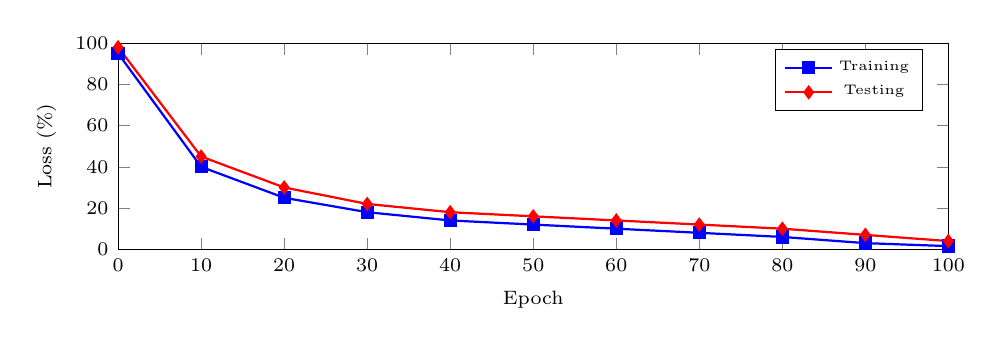
\begin{tikzpicture}
\begin{axis}[
  width=\linewidth, height=4.2cm,
  xlabel={Epoch}, ylabel={Loss (\%)},
  xmin=0, xmax=100, ymin=0, ymax=100,
  legend pos=north east, legend style={font=\tiny},
  label style={font=\scriptsize}, tick label style={font=\scriptsize}
]
\addplot[mark=square*, blue, thick] coordinates {
(0,95)(10,40)(20,25)(30,18)(40,14)(50,12)(60,10)(70,8)(80,6)(90,3)(100,1.55)
};
\addplot[mark=diamond*, red, thick] coordinates {
(0,98)(10,45)(20,30)(30,22)(40,18)(50,16)(60,14)(70,12)(80,10)(90,7)(100,4)
};
\legend{Training, Testing}
\end{axis}
\end{tikzpicture}
\caption{Training and testing loss curve of Mask R-CNN}
\label{fig6}
\end{figure}

Fig. 5 shows epochs on the x-axis and accuracy on the y-axis, comparing testing and training accuracy. Fig. 6 shows a loss curve plotted against epochs, indicating that the loss decreases as epochs increase. The proposed procedure yields an accurate result with a reasonably low loss of 1.55\%. With a low percentage of error, the proposed XXX model achieved 98.45\% training and testing accuracy across the number of epochs.

\subsection{Comparative analysis}
The effectiveness of the DL network was determined by comparing the proposed XXX model against four classifiers --- R-CNN, Fast R-CNN, Faster R-CNN, and Fully Convolutional Networks (FCN) --- as shown in Table~\ref{tab1}. A variety of measures were used to evaluate each DL technique's performance, including F1 score, accuracy, recall, specificity, and precision. The proposed XXX model has an accuracy of 98.45\%.

\begin{table}[htbp]
\caption{Comparison Between DL Networks and Proposed XXX Model}
\begin{center}
\begin{tabular}{@{}lccccc@{}}
\toprule
\textbf{Networks} & \textbf{Accuracy} & \textbf{Specificity} & \textbf{Precision} & \textbf{Recall} & \textbf{F1 score} \\
\midrule
R-CNN        & 93.65 & 90.04 & 94.23 & 92.21 & 90.25 \\
Fast R-CNN   & 95.28 & 94.58 & 91.04 & 95.05 & 91.48 \\
Faster R-CNN & 94.45 & 96.24 & 92.45 & 94.28 & 94.24 \\
FCN          & 97.07 & 92.56 & 95.27 & 90.75 & 93.75 \\
Mask RCNN    & \textbf{98.45} & \textbf{97.15} & \textbf{96.78} & \textbf{96.02} & \textbf{95.68} \\
\bottomrule
\end{tabular}
\label{tab1}
\end{center}
\end{table}

\begin{figure}[htbp]
\centering
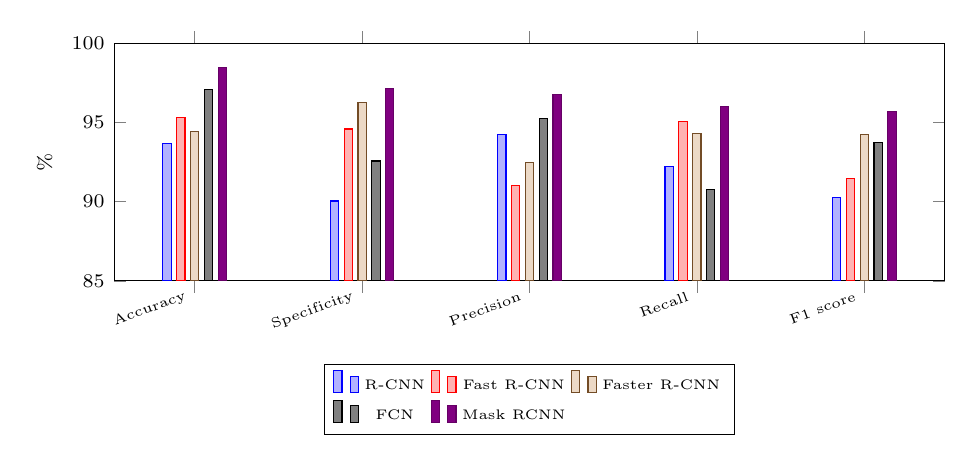
\begin{tikzpicture}
\begin{axis}[
  width=\linewidth, height=4.6cm,
  ybar, bar width=3pt,
  symbolic x coords={Accuracy,Specificity,Precision,Recall,F1 score},
  xtick=data, x tick label style={font=\tiny, rotate=20, anchor=east},
  ymin=85, ymax=100,
  ylabel={\%}, label style={font=\scriptsize}, tick label style={font=\scriptsize},
  legend style={font=\tiny, at={(0.5,-0.35)}, anchor=north, legend columns=3},
  enlarge x limits=0.12
]
\addplot coordinates {(Accuracy,93.65)(Specificity,90.04)(Precision,94.23)(Recall,92.21)(F1 score,90.25)};
\addplot coordinates {(Accuracy,95.28)(Specificity,94.58)(Precision,91.04)(Recall,95.05)(F1 score,91.48)};
\addplot coordinates {(Accuracy,94.45)(Specificity,96.24)(Precision,92.45)(Recall,94.28)(F1 score,94.24)};
\addplot coordinates {(Accuracy,97.07)(Specificity,92.56)(Precision,95.27)(Recall,90.75)(F1 score,93.75)};
\addplot coordinates {(Accuracy,98.45)(Specificity,97.15)(Precision,96.78)(Recall,96.02)(F1 score,95.68)};
\legend{R-CNN, Fast R-CNN, Faster R-CNN, FCN, Mask RCNN}
\end{axis}
\end{tikzpicture}
\caption{Graphic representation of performance analysis for Mask R-CNN}
\label{fig7}
\end{figure}

To compare several DL networks based on performance measures and determine an appropriate percentage of classification accuracy, Table~\ref{tab2} was examined. The proposed Mask R-CNN outperforms R-CNN, Fast R-CNN, Faster R-CNN, and FCN by 4.87\%, 3.21\%, 4.06\%, and 1.40\% respectively, in terms of overall accuracy range. Fig. 7 shows a graphic representation of the Mask R-CNN comparative evaluation.

\begin{table}[htbp]
\caption{Comparison of Existing Methods with the Proposed Method}
\begin{center}
\begin{tabular}{@{}p{4.3cm}p{2.1cm}c@{}}
\toprule
\textbf{Authors} & \textbf{Methods} & \textbf{Accuracy} \\
\midrule
Shen, Z., et al. (2024) \cite{b12} & DBSCAN & 96.30\% \\
Seemanthini, K. and Manjunath, S.S. (2018) \cite{b15} & Cluster segmentation & 89.59\% \\
Khan, D., et al. (2024) \cite{b17} & k-fold cross-validation & 97\% \\
Proposed & Mask RCNN & \textbf{98.45\%} \\
\bottomrule
\end{tabular}
\label{tab2}
\end{center}
\end{table}

According to Table~\ref{tab2}, the comparison of the suggested and existing methods is demonstrated. The proposed XXX model achieves an overall accuracy improvement of 2.18\%, 8.99\%, and 1.47\% compared to the existing methods such as DBSCAN, cluster segmentation, and k-fold cross-validation.

\section*{Acknowledgment}
With great appreciation, the author would like to thank the supervisor for his leadership and steadfast support during this project.

\section{Conclusion}

In this research, a novel virtual reality-based XXX model was proposed for tracking human motion to identify suspicious activity within an organization. The system uses various sensors such as cameras and motion sensors to capture real-world activity in a monitored space. These sensors capture continuous video, which has been converted into frames for further processing. The video frames are pre-processed using the bilateral filter to reduce noise while preserving edges. The Mask R-CNN model is used for human motion tracking from the frames, assigns bounding boxes around each detected human, and predicts segmentation masks on each detected frame. Mask R-CNN comprises multiple architectures, namely a backbone architecture such as ResNet-50, RPN, and RoI. The tracking data is stored in a database server and displayed on a large screen, allowing security personnel to observe activities in the monitored environment. The proposed Mask R-CNN outperforms Fast R-CNN, FCN, and Faster R-CNN by 3.21\%, 1.40\%, 4.87\%, and 4.06\% respectively, in terms of overall accuracy range. According to the result, the proposed model attains a 98.45\% accuracy rate for tracking human motion. The proposed XXX model achieves an overall accuracy improvement of 2.18\%, 8.99\%, and 1.47\% compared to the existing methods such as DBSCAN, cluster segmentation, and k-fold cross-validation. Moreover, future research directions include integrating emerging technologies like adversarial learning, domain adaptation, and multimodal fusion to improve accuracy, reliability, and fairness in real-world applications.

\begin{thebibliography}{00}
\bibitem{b1} B. Wang, J. C. Lu, and K. Zhang, ``Textile-based strain sensor for human motion detection,'' \textit{Energy Environ. Materials}, vol. 3, no. 1, pp. 80-100, 2020.
\bibitem{b2} A. Ahilan, and P. Deepa, ``A reconfigurable virtual architecture for memory scrubbers (VAMS) for SRAM-based FPGAs,'' \textit{Int. J. Appl. Eng. Res.}, vol. 10, no. 10, pp. 9643-9648, 2015.
\bibitem{b3} S. Reeba Rex, T. Pravin Rose, and S. Amudaria, ``Real-time remote monitoring via horse head optimization deep learning network,'' \textit{Int. J. Data Sci. Artif. Intell.}, vol. 02, pp. 42-47, 2024.
\bibitem{b4} Ramya Thatikonda, ``Predictive Monitoring Framework for Enhancing Operational Resilience in Retail Fulfillment Systems: A Case Study,'' \textit{Int. J. Syst. Design Comput.}, vol. 02, pp. 56-62, 2024.
\bibitem{b5} A. Ahilan, M. A. Rejula, S. N. Kumar, and B. M. Kumar, ``Virtual Reality Sensor-Based IoT Embedded System for Stress Diagnosis,'' \textit{IEEE Sensors J.}, 2023.
\bibitem{b6} V. Guzov, J. Chibane, R. Marin, Y. He, Y. Saracoglu, T. Sattler, and G. Pons-Moll, ``Interaction replica: Tracking human--object interaction and scene changes from human motion,'' \textit{2024 Int. Conf. 3D Vision (3DV)}, pp. 1006-1016, 2024.
\bibitem{b7} M.S. Ikbal, V. Ramadoss, and M. Zoppi, ``Dynamic pose tracking performance evaluation of HTC Vive virtual reality system,'' \textit{IEEE Access}, vol. 9, pp. 3798-3815, 2020.
\bibitem{b8} W. Mrabti, K. Baibai, B. Bellach, R.O.H. Thami, and H. Tairi, ``Human motion tracking: A comparative study,'' \textit{Proc. Comput. Sci.}, vol. 148, pp. 145-153, 2019.
\bibitem{b9} R. Kumar, M. Gupta, A. Agarwal, and A. Nayyar, ``CBAR-UNet: A novel methodology for segmentation of cardiac magnetic resonance images using block attention-based deep residual neural network,'' \textit{Multimed Tools Appl}, vol. 83, no. 37, pp. 85047--85063, Nov. 2024.
\bibitem{b10} A. Rudenko, L. Palmieri, M. Herman, K.M. Kitani, D.M. Gavrila, and K.O. Arras, ``Human motion trajectory prediction: A survey,'' \textit{Int. J. Robotics Res.}, vol. 39, no. 8, pp. 895-935, 2020.
\bibitem{b11} L.H. Chen, J. Zhang, Y. Li, Y. Pang, X. Xia, and T. Liu, ``Humanmac: Masked motion completion for human motion prediction,'' \textit{Proc. IEEE/CVF Int. Conf. Comput. Vision}, pp. 9544-9555, 2023.
\bibitem{b12} Z. Shen, J. Nunez-Yanez, and N. Dahnoun, ``Advanced Millimeter-Wave Radar System for Real-Time Multiple-Human Tracking and Fall Detection,'' \textit{Sensors}, vol. 24, no. 11, pp. 3660, 2024.
\bibitem{b13} A. Boonsongsrikul, and J. Eamsaard, ``Real-time human motion tracking by tello EDU drone,'' \textit{Sensors}, vol. 23, no. 2, pp. 897, 2023.
\bibitem{b14} Z. Liu, J. Huang, J. Han, S. Bu, and J. Lv, ``Human motion tracking by multiple RGBD cameras,'' \textit{IEEE Trans. Circuits Syst. Video Technol.}, vol. 27, no. 9, pp. 2014-2027, 2016.
\bibitem{b15} K. Seemanthini, and S.S. Manjunath, ``Human detection and tracking using HOG for action recognition,'' \textit{Proc. Comput. Sci.}, vol. 132, pp. 1317-1326, 2018.
\bibitem{b16} M.P. Wilk, M. Walsh, and B. O'Flynn, ``Low cost embedded multimodal opto-inertial human motion tracking system,'' \textit{2020 31st Irish Signals Syst. Conf. (ISSC)}, pp. 1-6, 2020.
\bibitem{b17} D. Khan, M. Alonazi, M. Abdelhaq, N. Al Mudawi, A. Algarni, A. Jalal, and H. Liu, ``Robust human locomotion and localization activity recognition over multisensory,'' \textit{Front. Physiol.}, vol. 15, pp. 1344887, 2024.
\bibitem{b18} A. Aalerud, and G. Hovland, ``Dynamic Augmented Kalman Filtering for Human Motion Tracking under Occlusion Using Multiple 3D Sensors,'' \textit{2020 15th IEEE Conf. Ind. Electron. Appl. (ICIEA)}, pp. 533-540, 2020.
\bibitem{b19} M. Nallasivam, and V. Senniappan, ``Moving human target detection and tracking in video frames,'' \textit{Studies inform. Control}, vol. 30, no. 1, pp. 119-129, 2021.
\bibitem{b20} A.K. Patil, A. Balasubramanyam, J.Y. Ryu, P.K. BN, B. Chakravarthi, and Y.H. Chai, ``Fusion of multiple lidars and inertial sensors for the real-time pose tracking of human motion,'' \textit{Sensors}, vol. 20, no. 18, 5342, 2020.
\bibitem{b21} S. Yue, ``Human motion tracking and positioning for augmented reality,'' \textit{J. Real-Time Image Process.}, vol. 18, no. 2, pp. 357-368, 2021.
\end{thebibliography}

\end{document}
